% =============================================================================================
% STANDALONE EXPORT OF §7 FOR EXTERNAL COLD REVIEW.
%
% Contains §7 exactly as it stands in main.tex. Nothing is re-typed for this export, so it cannot
% drift from the manuscript. §7 carries no figures of its own; the one figure it points at
% (Figure 7, coverage) belongs to §5 and is reproduced at the end for reference only.
%
% Build:  tectonic -X compile paper/review_s7.tex
% =============================================================================================
\documentclass[10pt]{article}
\usepackage{preprint}

\author{}
\date{}

\begin{document}

% §7 references six things outside this export. Bind each label to the number it carries in the
% manuscript so every reference resolves to what a reader of the full paper would see.
\makeatletter
\@namedef{r@sec:mechanism}{{3}{1}{Mechanism}{section.3}{}}
\@namedef{r@sec:mechanism@cref}{{[section][3][]3}{1}}
\@namedef{r@sec:mech-fix}{{3.6}{1}{Intervention}{subsection.3.6}{}}
\@namedef{r@sec:mech-fix@cref}{{[subsection][6][3]3.6}{1}}
\@namedef{r@sec:setup}{{4}{1}{Experimental design}{section.4}{}}
\@namedef{r@sec:setup@cref}{{[section][4][]4}{1}}
\@namedef{r@sec:results}{{6}{1}{Results}{section.6}{}}
\@namedef{r@sec:results@cref}{{[section][6][]6}{1}}
\@namedef{r@sec:repro}{{8}{1}{Reproducibility and verification}{section.8}{}}
\@namedef{r@sec:repro@cref}{{[section][8][]8}{1}}
\@namedef{r@app:claims}{{C}{1}{Claims audit}{appendix.C}{}}
\@namedef{r@app:claims@cref}{{[appendix][3][]C}{1}}
\makeatother

\setcounter{section}{6}   % so §7 numbers as §7, matching the manuscript
\setcounter{figure}{6}    % Figures 1--6 precede this section
\setcounter{table}{0}

{\centering
{\normalsize\textsc{Section 7 --- export for external review}}\\[0.5em]
{\Large\bfseries Capacity Eviction in Reconstruction-Trained Tokenizers}\\[0.4em]
{\small\color{tolgrey} Draft of \today\ --- section text frozen pending review}\\[1.6em]
}

\noindent\textbf{Note to the reviewer.} This is \S7 of a paper in preparation, exported verbatim
from the manuscript. Numbering matches: \S7.1--\S7.9. The pre-registered experiment has \emph{not}
been executed, so \S6 contains no results and nothing in \S7 is written with knowledge of an
outcome --- every limitation here was known and written before any number existed. References to
\S3, \S4, \S6, \S8 and Appendix~C point outside this export and are bound to their manuscript
numbers; \cref{fig:coverage} belongs to \S5 and is reproduced at the end for reference.

\medskip
\noindent\textbf{Ordering principle.} The subsections are ordered by what we believe a referee
would attack first, not chronologically and not by severity as we perceive it. The first three
bound what the paper may claim \emph{even if every pre-registered clause passes}. If that ordering
is wrong --- if something in \S7.5--\S7.9 belongs above something in \S7.1--\S7.4 --- that is
itself a useful finding.

\medskip
\noindent\textbf{What we would most like challenged.} (i) Whether \S7.1 concedes enough: the
headline mechanism is measured on a synthetic fixture, and we claim the entropy match licenses the
construction without claiming it reproduces real covariance geometry. (ii) Whether the required
disclosure in \S7.2 is sufficient, or whether a comparison with no external anchor should not be
reported at all. (iii) Whether \S7.3's unquantified capacity handicap is a disclosure or a hole ---
we state that $\Delta\text{IR}(4-5)$ mixes information with capacity and do not decompose them.
(iv) Whether \S7.4's power discussion is honest about a minimum detectable effect two orders of
magnitude above the prior. (v) Whether \S7.6's argument --- that signed returns are the only
channel a label leak travels on --- actually holds, since it is the weakest link in the validation
geometry and we know it. (vi) Anything a referee would raise that is not here at all.

\bigskip
\hrule
\bigskip

% =============================================================================================
% §7 Limitations.  Ordered by what a referee would attack first, not chronologically.
% Every number carries its artifact.  Nothing here is hedged into vagueness: a limitation stated
% imprecisely is not a disclosure.
% =============================================================================================
\section{Limitations}
\label{sec:limitations}

The limitations below are stated at the same confidence as the contributions, and in the order a
sceptical reader should apply them. Three of them --- the synthetic basis of the mechanism, the
absent external baseline, and the placebo's capacity confound --- bound what the paper is entitled
to claim even if every pre-registered clause passes.

\subsection{The mechanism is measured on a synthetic fixture, not on markets}
\label{sec:lim-fixture}

Everything in \cref{sec:mechanism} is measured on a constructed fixture. That is a deliberate
trade and it cuts both ways. The fixture's non-signal structure is entropy-matched to the real
lake --- a per-dimension deficit of $0.4631$ nats, reproduced at $0.462$ against a declared
tolerance of $0.05$ --- and its signal dimension is planted with an exactly computable information
content, which is what allows us to say that $94.4\%$ of a known quantity was recovered rather
than that a loss curve moved.
% artifact: runs_manifest/m6_interface_respec_design_pass.json :: filler_calibration.{lake_measurement.per_dim_deficit_nats=0.4631, achieved_per_dim_deficit_nats=0.462, tolerance_nats=0.05, within_tolerance=true}
It is also precisely what stops the result being a measurement of markets. We do not know the
variance and covariance geometry of real trade-flow imbalance against real price well enough to
assert that the fixture reproduces it; we know only that one entropy statistic matches.

The consequence is a specific one, and we hold to it under every experimental outcome: capacity
eviction is a mechanism we demonstrate, not a market phenomenon we measure, and it is not this
paper's headline claim. A reader who wants the mechanism established on real microstructure will
not find it here. What the pre-registered ablation of \cref{sec:setup} tests is the downstream
question --- whether real trade-flow imbalance survives the re-specified pipeline --- and a
positive result there would be consistent with the mechanism without confirming it, because many
other differences between cells 2 and 4 could produce the same sign.

Two narrower limits inside the same fixture. We demonstrate the effect for one reconstruction
objective, one quantizer family and one class of encoder. We show that \emph{this} objective
allocates by variance and covariance; we do not show that no reconstruction objective can do
otherwise, and \cref{sec:mech-fix} is a counterexample to the strong form --- it is a
reconstruction objective that carries the evicted channel, because it was given an explicit term
to do so. Separately, the $94.4\%$ recovery figure is calibrated against a single matched
reference run and inherits whatever run-to-run variation that reference carries; we report it as
one measurement, not as an expectation over runs.
% artifact: runs_manifest/m6_token_control_run_manifest.json :: decision_inputs.{H0_source, H0_val=13.5979, final_val_minus_H0=-0.8496}

\subsection{The BSQ baseline is ours, and nothing external anchors it}
\label{sec:lim-baseline}

Cell 1 --- binary spherical quantization on OHLCV-only inputs --- is our own implementation at
matched bits per token. It is not an independently validated reference. The evaluation harness was
originally specified to load published reference weights and reproduce their reported rank
information coefficient as an external anchor for this cell. That gate was found unexecutable and
dropped as binding before any cell was scored, for three separate reasons, each sufficient on its
own: the reference paper publishes two rank information coefficients for the same model that
differ by $2.4\times$ ($0.0431$ against $0.0665$) without the pre-registration saying which
applies; both are measured on Shanghai Stock Exchange $15$-minute equity bars, a market and a
frequency this study firewalls out of v1, so the gate's two requirements --- reproduce the
published number, and do it on our own pinned slice --- cannot both hold; and executing the
weights would require importing the reference model code, which our independence invariant
forbids. Resolvability was never the obstacle: the band is $4.51$ to $11.05$ standard errors wide
at the measured effective sample size of $1{,}401{,}637$.
% artifact: src/trikaal/eval/external_validation.py :: GATE_IS_BINDING = False, and the three-count comment above it
% artifact: runs_manifest/m6_c4_resolvability.json :: which_published_figure.{ic_price_series=0.0431, ic_return_forecasting=0.0665, dataset_in_the_caption}; resolvability_MEASURED.{n_eff_summed=1401637, se_rankic=0.0008446, band_over_se_price_series=4.51, band_over_se_return_forecast=11.05}

Two compensating controls were armed in its place, and it is important to be exact about what they
do. A saturation check asks whether cell 1 was trained enough to be a fair baseline. A codebook
utilization gate, pinned at $0.95$, asks whether our BSQ codebook collapsed. Neither answers the
question the external gate was for. We therefore carry the following sentence as a required field
of every verdict manifest, refused if absent, and reproduce it verbatim here:

\begin{quote}
We therefore cannot exclude that our BSQ baseline is weaker than a reference BSQ implementation,
which would inflate the FSQ-vs-BSQ comparison reported in \cref{sec:results}.
\end{quote}
% artifact: src/trikaal/eval/external_validation.py :: BSQ_DISCLOSURE (verbatim); conformance PINNED_CODEBOOK_MIN_UTILIZATION = 0.95

This bounds the quantizer leg specifically. It does not bound the input-arm leg: the comparison
between cells 2 and 4, and between cell 4 and the placebo, is internal to our own implementation
on both sides, and a weak baseline cannot inflate a difference in which the same baseline appears
twice.

The consequence is a withdrawal, and we make it here rather than leaving it implicit. \textbf{The
three marginals involving a BSQ arm --- $\IR(2) - \IR(1)$, $\IR(4) - \IR(3)$, and $\IR(3) -
\IR(1)$ --- are reported, not claimed.} They appear in \cref{sec:results} with their confidence
intervals because suppressing them would be worse, and they are excluded from every claim this
paper makes. A reader who wants the FSQ-versus-BSQ question answered will not find it answered
here; what is answered is the input-arm question, on which the same implementation stands on both
sides of every comparison.

\subsection{The placebo removes information and capacity together}
\label{sec:lim-placebo}

The shuffled-microstructure cell is the design's central control, and its reach is narrower than
its name suggests. Measured on the fixture, the shuffle destroys exactly what it was built to
destroy: microstructure's contemporaneous link to price falls from $0.2037$ to $0.0005$, and its
own lag-1 autocorrelation from $0.4165$ to $0.0006$, while the within-block and within-OHLCV
correlations are left as they were.
% artifact: docs/m6_c12_placebo_mechanism.md — the measured before/after table, parsed at render time by paper/figures/make_fig5_design.py

But microstructure dimensions in cell 4 are partly amortized against structure the code already
carries, and shuffling removes that sharing along with the information. $\Delta\IR(4-5)$ is
therefore (information) $+$ (capacity handicap), and \textbf{we have not quantified the handicap in
information-ratio units}. A sixth cell holding the microstructure block constant rather than
shuffled would bracket it, and no such cell appears anywhere in the pre-registration --- we have
verified this by exhaustive search of that document --- so it is future work, not a committed
contingency we chose not to exercise. The practical consequence: a positive $\Delta\IR(4-5)$ is
evidence that microstructure carries information beyond input capacity, and is not a calibrated
estimate of how much.

\subsection{The effect we can detect is larger than the effect we expect}
\label{sec:lim-power}

At the headline horizon the paired minimum detectable effect is $3.518$ annualized information
ratio, against an economic materiality floor of $0.5$.
% artifact: runs_manifest/m6_mde_inputs.json :: h15_pooled.{MDE_annualized_IR=3.518, T=35063, T_eff=35002.3, N_breadth_eff=1.5, avg_breadth=40.0}
% artifact: src/trikaal/eval/verdict.py :: ECON_FLOOR_IR = 0.5
The only prior we hold for the quantity under test is our own univariate liveness screen of
trade-flow imbalance on a single symbol: $|\text{RankIC}| = 0.0270$ at $h=5$ and $0.0197$ at the
headline $h=15$, both with confidence intervals excluding zero. That screen's own source describes
it as a liveness screen and not the headline test, and we use it here only to set expectations
about magnitude.
% artifact: docs/milestone2_btcusdt_stage1.md — TFI RankIC -0.0270 [-0.0304,-0.0236] at h=5; -0.0197 [-0.0230,-0.0166] at h=15; BTCUSDT only
An effect of that size does not become an information ratio of $3.5$. We therefore state plainly,
before seeing any result, that a null or inconclusive outcome is the most likely honest one, and
that this was pre-committed as publishable: the outcome taxonomy has three members, and the
decision rule names what we report under each.

A second, less visible power limitation. The minimum detectable effect above is built from
\emph{scoring} noise --- the dispersion of the portfolio return series --- and contains no term
for training variance. That omission is not conservative, and we found its magnitude by accident:
two runs at the same seed, the same recipe, the same horizon and the same estimator produced
fraction-negative $0.5662$ and $0.99883$ for the same cell. Same-seed divergence is basin-hopping,
and it is a lower bound on across-seed variance, which is the quantity the design actually
averages over. Five seeds are pinned up front, which helps; forcing deterministic kernels does not
help, because it removes the same-seed component and leaves the across-seed component untouched.
% artifact: docs/m6_prereg.md §7 v1.4.5 — acceptance cell4 frac_negative 0.5662 vs money-leg cell4 0.99883 at identical h/cap/estimator/seed/recipe
% artifact: src/trikaal/eval/conformance.py :: PINNED_SEEDS = (0,1,2,3,4)

What we do about it is a refusal rather than a correction. A power guard, computed after the
clauses and unable to alter them, compares each cell's across-seed range against the effect being
claimed; if the range reaches the claimed effect, the verdict is reported as
\textsc{halt\_adjudicate} rather than as an outcome. The guard is HALT-only by construction --- it
can manufacture neither a positive nor a negative claim --- which is what makes it legitimate to
have added it before the run. It does not increase power. It prevents us from reporting a number
smaller than its own inputs' wobble.
% artifact: src/trikaal/eval/verdict.py :: power_guard; tests/eval/test_degeneracy_guard.py

\subsection{Whether the execution filter binds on real data is unmeasured}
\label{sec:lim-filter}

The headline metric is a cost-aware net information ratio \emph{under a forecast-magnitude
execution filter}, $\theta = \kappa c$. Whether that filter does any per-bar work on real data is
not known, and nothing in this project measures it: no evaluation artifact from a real-lake run
retains a decision-activity value, so the question is genuinely open rather than answered
elsewhere. On the calibration fixture it behaved in both extremes --- inert on the degenerate
checkpoints at the pinned horizon, and binding at every $\kappa$ on a non-degenerate one
(\cref{sec:metric}).

The reason this is a limitation and not a detail is arithmetic. Binding is decided by the
\emph{forecast} magnitude, and for a calibrated conditional mean
$\operatorname{std}(\hat{\mu}) = \text{IC}\cdot\operatorname{std}(y)$. The $15$-bar forward return
has a standard deviation of $0.004238$ on our largest instrument and a $192$-instrument median of
$0.00536$; at our own prior of $|\text{RankIC}| = 0.027$ the threshold sits between seven and
twenty-eight standard deviations out in the forecast distribution across the modeled-cost range,
and one instrument in $192$ would trade even $5\%$ of bars at the most favourable cost. If the
trained models are calibrated, activity is near zero everywhere. If they are over-dispersed, they
trade, but the realized information ratio then partly reflects miscalibration rather than skill.
% artifact: measured on processed/universe_bars — BTCUSDT 15-bar forward log-return std = 0.004238
%   over n = 1,051,199; 192-instrument median 0.00536 (p5 0.00372, p95 0.00887), 2024-06.
%   theta = kappa * c_modeled per src/trikaal/eval/xsection.py:335; modeled c_total range 8e-4 to
%   2.1e-3 per the harness KATs. Arithmetic over measured inputs; the harness was not run at these
%   values.

The pre-registration does not assume an answer. A HALT-only degeneracy guard refuses a verdict for
any cell whose decision activity at $\kappa^\ast$ is exactly $0$ or $1$, tested on the seed mean
and on every individual seed. We state its limit rather than leave it to be found: unlike the
companion sign-balance test, which carries a $[0.05, 0.95]$ band, the activity test fires only at
the exact endpoints, so an activity of $0.999$ passes it. Whether to band that leg is an open
decision at the time of writing, and \cref{app:repro} records it as open rather than resolved.
% artifact: src/trikaal/eval/verdict.py :: FRAC_NEG_BAND = (0.05, 0.95) on the sign leg;
%   _never_binds tests v <= 0.0 or v >= 1.0 on the activity leg. No amendment supersedes this.

\subsection{One exchange, one venue, one year of scored data}
\label{sec:lim-universe}

The lake is $304{,}625{,}181$ one-minute bars across $200$ instruments, and the breadth of that
number should not be read as breadth of evidence. Every instrument is a USDT-margined perpetual
future on a single exchange. Perpetuals are not spot, and one exchange is not the market: fee
schedules, tick sizes, liquidation mechanics and the composition of flow all differ across venues,
and trade-flow imbalance is a venue-local quantity in a way that returns are not. Nothing here
establishes that the result transfers to spot, to another exchange, to dated futures, or to any
other asset class.

Within that universe the scored slice is narrower still. The headline metric is computed on $40$
instruments, not $200$, and on forward blocks $1$ through $5$ --- roughly 2024-01-01 to
2025-01-01, one year --- with block $0$ spent selecting the execution filter and excluded. The
remaining $160$ instruments are lake breadth, not evaluation breadth.
% artifact: runs_manifest/m6_mde_inputs.json :: symbols_sampled (40 entries), primary_region_ms = [1704132000000, 1735689600000], n_blocks = 6
One year of scored data at a $15$-bar horizon is $35{,}063$ periods per instrument, and the
effective breadth across a correlated $40$-instrument cross-section is $1.5$, not $40$ --- which
is where most of the minimum detectable effect in \cref{sec:lim-power} comes from. That single
year is also one market regime. We do not test regime transfer and cannot claim it.

Survivorship is owned rather than filtered: instruments that stop trading are retained, and $17$
of them stop inside the window, giving the ragged right edge of \cref{fig:coverage}. This removes
one bias; it does not remove listing bias, since an instrument must have been listed on this venue
to enter the universe at all.
% artifact: runs_manifest/m6_c15b_lake_surface_check.json :: bars = 304625181; paper/figures/make_fig7_coverage.py — enumerated from processed/universe_bars at render time

\subsection{The embargo premise is established for one channel only}
\label{sec:lim-embargo}

The $120$-bar leading embargo is a $60$-bar label look-forward plus a $60$-bar
serial-correlation margin, and the premise behind the second margin was measured on all $200$
instruments rather than assumed, with a control arm that recovers a known AR(1) answer first so
that a null reading is a measurement and not a silent failure. For signed returns it holds
comfortably: autocorrelation at lag $60$ is $0.0067$ on average and $0.0191$ at the worst
instrument.

For absolute returns it does not hold: $0.2323$ on average and $0.3604$ at the worst instrument,
at the same lag. We report this as a red finding rather than a footnote. Our position is that
signed returns are the channel a label leak would actually travel on --- the labels are signed
forward returns, and a leak means a training window seeing the sign of a future return it should
not --- and that persistent absolute-return autocorrelation is volatility clustering, a
well-established property of the series that is present in the training region and the evaluation
region alike and is not a path from label to feature.

That is an argument, and it is the weakest link in the validation geometry. What we have
established is that the signed channel is clean at the chosen margin. What we have \emph{not}
established is that no leakage path exists through volatility --- for instance, a model that
learns to condition on realized volatility could in principle be advantaged by a training window
whose volatility state persists into the evaluation region. Extending the margin until the
absolute-return premise also holds would require a margin several times longer and would cost
evaluation data we do not have; we chose the shorter margin and we are stating the choice.
% artifact: runs_manifest/m6_c20_embargo_premise.json :: reading.{H_MAX_DEFAULT=60, L_CORR_DEFAULT=60, EMBARGO_DEFAULT=120, ALL200_signed_acf_at_60_mean=0.006669, ALL200_signed_acf_at_60_worst=0.019079, abs_acf_at_L_corr_60_mean=0.2323, abs_acf_at_L_corr_60_worst_symbol=0.3604, premise_supported_for_ABS_returns=false}; control_arm.series = AR(1) rho=0.97, n=200000

\subsection{The microstructure leg is narrower than ``microstructure'' suggests}
\label{sec:lim-features}

\paragraph{Trade-flow imbalance, not order-flow imbalance.}
The imbalance signal is computed from freely available aggregated trades, and is therefore signed
\emph{executed-volume} imbalance. True order-flow imbalance requires order book depth --- the
arrival and cancellation of resting liquidity --- which we do not have. The distinction is not
cosmetic: order-flow imbalance carries information about intent that never executes, and a
substantial part of the microstructure literature's predictive content comes from exactly that.
We use the name trade-flow imbalance everywhere, in code, configuration and prose, and a negative
result here is evidence about trade-flow imbalance only. Depth-based order-flow imbalance is
explicit v2 work.

\paragraph{Three of sixteen feature dimensions are structurally absent.}
The per-bar feature vector is specified as $16$ dimensions, of which $13$ are live. Funding rate
and open interest occupy dimensions $13$ through $15$; they are wired, carried through the
pipeline, and masked --- and in the v1 lake they have standard deviation exactly $0.0$ and are
masked on $100\%$ of all $304{,}625{,}181$ bars, because ingest covers klines and aggregated
trades only. They are specified and structurally absent. The microstructure block that the
ablation actually varies is six live dimensions, $7$ through $12$, each non-degenerate across all
$200$ instruments.
% artifact: docs/m6_prereg.md §7 v1.6.16 — x_13/14/15 stddev exactly 0.0, m_13/14/15 masked on 100% of bars
% artifact: src/trikaal/constants.py :: MASK_BITS_PERP = (13, 14, 15)
% artifact: runs_manifest/m6_c10_micro_density.json :: symbols_with_zero_unmasked_per_dim = {} for dims 7-12; per_dim_total_unmasked ~ 3.0e8 each
Funding and open interest are the two channels most plausibly carrying the information a
perpetual-futures microstructure study would want, and the study is run without them. This is a
limitation of the v1 data, not a design choice defended on merit.

\subsection{Two matching caveats}
\label{sec:lim-matching}

\paragraph{$\lambda$ is fitted to a synthetic proxy.}
The class weight that makes the per-bar bottleneck carry the microstructure block was selected on
the calibration fixture, not on real data, and its acceptance threshold was restated after
calibration results were seen --- we state that plainly in \cref{sec:mech-fix} rather than let it
be discovered. It is pinned pre-data at a single value and applied identically to every arm, so it
cannot favour any cell relative to any other. The residual risk is that the proxy does not
transfer: a $\lambda$ tuned for a synthetic covariance geometry may under-serve the real one. The
guard is the legibility gate, which is why it exists --- it is evaluated on real data before any
second-stage training begins, requires at least $0.90$ sign accuracy on every one of the six live
microstructure dimensions with no mean clause and no floor, and raises a hard stop rather than
degrading quietly. A gate that fires costs us the run; it does not cost us the honesty of the
result.

\paragraph{The arms are matched to $0.327\%$, not exactly.}
The backbone realizes $21{,}301{,}248$ parameters at the FSQ vocabulary and $21{,}231{,}616$ at
the BSQ vocabulary --- $69{,}632$ fewer, or $0.327\%$ --- because embedding and output-head rows
scale with vocabulary size. The two quantizer arms also differ by $0.058$ bits per bar. Both gaps
favour the FSQ arm, both are an order of magnitude smaller than any effect the design can detect,
and both are reported rather than absorbed. We do not claim exact parameter parity; we claim
parity to a stated tolerance, hard-checked before any cell is scored.
% artifact: runs_manifest/m6_cuda_probe.json :: params_gate = "21,301,248 enforced by OrchestratorConfig.expect_backbone_params"

\subsection{Reproducibility is bit-exact except in one place, and that place is training}
\label{sec:lim-determinism}

The data pipeline, the frozen normalization statistics and prediction replay are bit-exact from
one configuration file, a pinned seed and content-hashed inputs. GPU training is not, unless the
deterministic-attention fallback is enabled, and the two are not the same claim: deterministic
attention is necessary for bit-exact training and is not sufficient, because reduction order
elsewhere in the backward pass is unconstrained. We record the mode for every run.
\Cref{sec:repro} states exactly which artifacts carry which guarantee, and \cref{app:claims}
separates what was measured from what was estimated across the whole paper.


\clearpage
\begin{figure}[t]
  \centering
  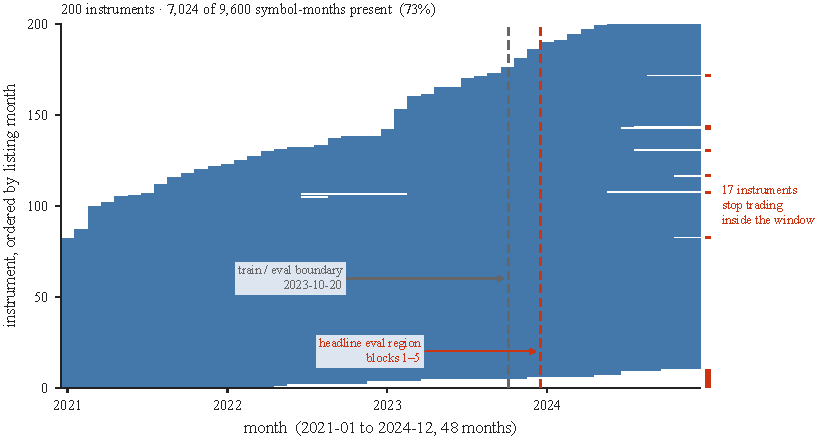
\includegraphics[width=\textwidth]{figures/fig7_coverage.pdf}
  \caption{\textbf{Reproduced from \S5 for reference only} --- \cref{sec:lim-universe} points at
  this panel. Month-by-month presence for all $200$ instruments over the four-year window, ordered
  by listing month: $7{,}024$ of a possible $9{,}600$ symbol-months are present. The right edge is
  ragged because instruments that stop trading are \emph{kept}, and $17$ of them stop inside this
  window.}
  \label{fig:coverage}
\end{figure}

\clearpage
\bibliographystyle{plainnat}
\bibliography{refs}

\end{document}
